\documentclass{beamer}

\mode<presentation> {

%\usetheme{default}
%\usetheme{AnnArbor}
%\usetheme{Antibes}
%\usetheme{Bergen}
%\usetheme{Berkeley}
%\usetheme{Berlin}
%\usetheme{Boadilla}
%\usetheme{CambridgeUS}
%\usetheme{Copenhagen}
%\usetheme{Darmstadt}
%\usetheme{Dresden}
%\usetheme{Frankfurt}
%\usetheme{Goettingen}
%\usetheme{Hannover}
%\usetheme{Ilmenau}
%\usetheme{JuanLesPins}
%\usetheme{Luebeck}
\usetheme{Madrid}
%\usetheme{Malmoe}
%\usetheme{Marburg}
%\usetheme{Montpellier}
%\usetheme{PaloAlto}
%\usetheme{Pittsburgh}
%\usetheme{Rochester}
%\usetheme{Singapore}
%\usetheme{Szeged}
%\usetheme{Warsaw}


%\usecolortheme{albatross}
%\usecolortheme{beaver}
%\usecolortheme{beetle}
%\usecolortheme{crane}
%\usecolortheme{dolphin}
%\usecolortheme{dove}
%\usecolortheme{fly}
%\usecolortheme{lily}
%\usecolortheme{orchid}
%\usecolortheme{rose}
%\usecolortheme{seagull}
%\usecolortheme{seahorse}
%\usecolortheme{whale}
%\usecolortheme{wolverine}

%\setbeamertemplate{footline} % To remove the footer line in all slides uncomment this line
%\setbeamertemplate{footline}[page number] % To replace the footer line in all slides with a simple slide count uncomment this line

%\setbeamertemplate{navigation symbols}{} % To remove the navigation symbols from the bottom of all slides uncomment this line
}

\usepackage{graphicx} % Allows including images
\usepackage{booktabs} % Allows the use of \toprule, \midrule and \bottomrule in tables
\usepackage{amsfonts}
\usepackage{mathrsfs}
\usepackage{amsmath,amssymb,graphicx, bm}

%----------------------------------------------------------------------------------------
%	TITLE PAGE
%----------------------------------------------------------------------------------------

\title["5.4"]{5.4: Forecasting}

\author{Taylor} 
\institute[UVA] 
{
University of Virginia \\
\medskip
\textit{} 
}
\date{} 

\begin{document}
%----------------------------------------------------------------------------------------

\begin{frame}
\titlepage 
\end{frame}
%----------------------------------------------------------------------------------------

\begin{frame}
\frametitle{Motivation}

After you've estimated the models parameters, you can use those to forecast future data with one of the algorithms we learned in 3.3. That's what this chapter is about.
\newline

We skipped section 3.3, however, so we won't be deriving our predictors specifically using the innovations algorithm. 


\end{frame}


%----------------------------------------------------------------------------------------

\begin{frame}
\frametitle{Example 5.4.1}

We are assuming the estimated model is true here.
\[
X_t + 4.035 = Z_t - .818 Z_{t-1}
\]
Then
\begin{align*}
\hat{X}_{t+h} &= - 4.035 + E[Z_{t+h}|X_{1:t}] - .818 E[Z_{t+h-1}|X_{1:t}] \\
&= 
\begin{cases}
-4.035 -.818(X_t - \hat{X}_t) & h=1 \\
-4.035 & h > 1
\end{cases}
\end{align*}


\end{frame}

%----------------------------------------------------------------------------------------

\begin{frame}[fragile]
\frametitle{Example 5.4.1}

See code handout for more details.

\begin{verbatim}
> forecast(x = x, xv = NULL, a = mod, opt=2)
 Step     Prediction      sqrt(MSE)    Lower Bound    Upper Bound
    1       1.003845       45.15743      -87.50472       89.51242
    2   8.715312e-16       58.34096      -114.3483       114.3483
    3   8.715312e-16       58.34096      -114.3483       114.3483
\end{verbatim}

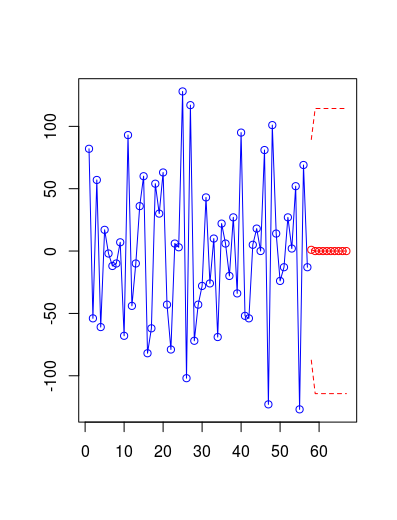
\includegraphics[width=45mm]{/home/taylor/UVa/all_teaching/4170_slides/5/5.4/pics/forecast1.png}

\end{frame}

%----------------------------------------------------------------------------------------

\begin{frame}[fragile]
\frametitle{Out-of-Sample Prediction}

In finance, you are usually primarily concerned with out-of-sample forecasting. Here are some things to consider:

\begin{enumerate}
\item You are always uncertain about the model (more on this next chapter)
\item Even if you have the model right, your estimates for the parameters are random and are going to be off. 
\item Even if you have the right model and parameters, there is no reason for this to be a good model forever.
\end{enumerate}

*Theoretically* more data usually solves the first two problems. However, *in practice* more data magnifies the third problem.



\end{frame}






\end{document} 